\documentclass{standalone}
\usepackage{pgfplots}

\begin{document}

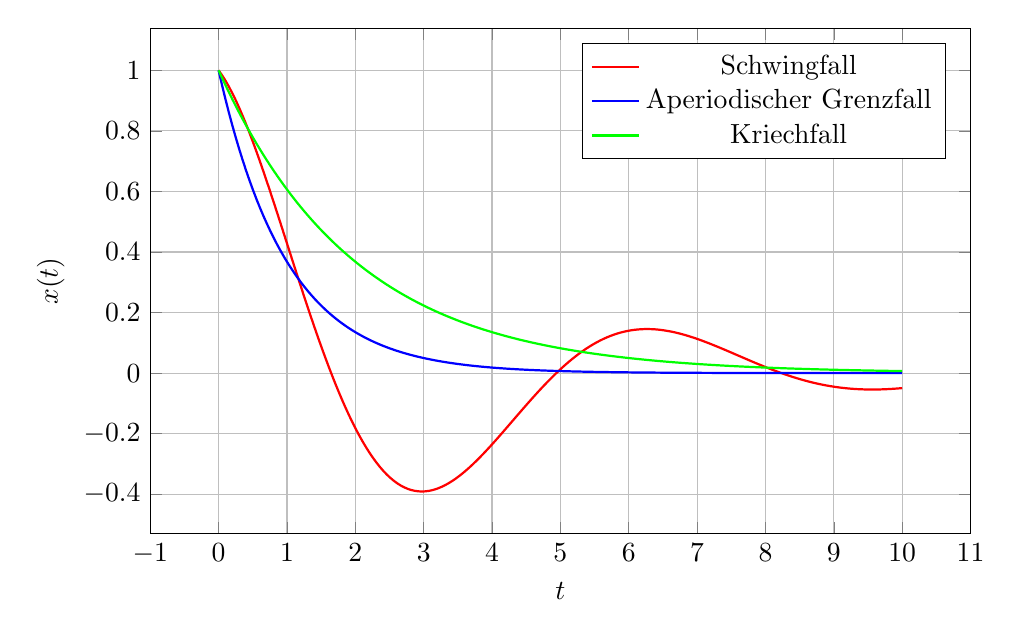
\begin{tikzpicture}
    \begin{axis}[
        xlabel={$t$},
        ylabel={$x(t)$},
        grid=major,
        width=12cm,
        height=8cm,
        legend pos=north east,
        samples=200,
        domain=0:10,
    ]

    % Unterdämpfung: zeta < 1 (rot)
    \addplot[color=red, thick] 
        {exp(-0.3*x) * cos(deg(sqrt(1-0.3^2) * x))};
    \addlegendentry{Schwingfall}

    % Aperiodischer Grenzfall: zeta = 1 (blau)
    \addplot[color=blue, thick] 
        {exp(-x)};
    \addlegendentry{Aperiodischer Grenzfall}

    % Kriechfall: zeta > 1 (grün)
    \addplot[color=green, thick] 
        {exp(-0.5*x)};
    \addlegendentry{Kriechfall}


    \end{axis}
\end{tikzpicture}

\end{document}
